\scanpage{45}
% archive foliation: 44
prenne le det du faisceau descendu, on trouve à partir d'un faisceau \unsure{rel. ample|très ample} sur $X/Y$, un faisceau ample sur $f_*(X/T)/f_*(Y/T)$ \deleted{\unsure{etc}}]. Kif-kif pour propre.

\uline{Proposition} Soit $g:X/T\longrightarrow Y/T$ un morphisme, et soit $\uline{L}$ un faisceau inversible sur $X$ \uline{ample} \deleted{pour} (resp. très ample) pour $g$. Alors $\det f_*(\uline{L})$ est un faisceau ample (resp. très ample) pour
\[
f_*(X/T)\longrightarrow f_*(Y/T)
\]
Démonstration. \textcircled{2} On peut supposer $Y$ affine, l'amplitude \deleted{\unsure{est un caractère}} étant une notion locale. \unsure{(1)} On \deleted{\unsure{est ramené}} \inserted{est ramené au cas ``ample''.} \deleted{\unsure{que ce résultat}} De plus, on est ramené à prouver ceci: Si $X=\unsure{P|\mathbf P}_Y^n$, et $\uline{L}$ le faisceau fondamental dessus, alors $f_*(\uline{L}/T)$ \deleted{est} définit une immersion projective fermée de $f_*(\unsure{P|\mathbf P}_Y^n)$ sur \unsure{ce qui est} $f_*(Y/T)$. Mais utilisant la commutation de $f_*$ aux \unsure{produits|chg. de base}, on est ramené au cas où $Y=T$. De plus, la question étant locale, on peut supposer $S$ affine $=\operatorname{Spec}(A)$, $T=\operatorname{Spec}(B)$, $B$ étant libre de type fini (rang $d$) sur $A$.
\margin{\figure{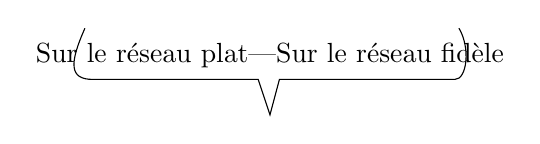
\begin{tikzpicture}[baseline=(m.base)]
\node[inner sep=3pt] (m) at (0,0) {\unsure{Sur le réseau plat|Sur le réseau fidèle}};
\draw (-2.35,0.35)..controls(-2.55,-0.1)and(-2.55,-0.3)..(-2.25,-0.3)--(-0.15,-0.3)--(0,-0.75)--(0.12,-0.3)--(2.35,-0.3)..controls(2.5,-0.3)and(2.55,0.1)..(2.4,0.35);
\end{tikzpicture}}}
\margin{$\unsure{f_*(U/T)\longrightarrow f_*(X/T)}$}
\margin{$S\qquad T$}
\margin{\deleted{N.B. \unsure{Rien de si simple|Rien de plus simple} si on introduit sur $Y$ le foncteur $f_*(\uline{L})$ (qui \unsure{n'est pas de} type fini en général) pour \uline{\unsure{pourquoi|prouver}} (i) \unsure{les puissances|que le faisceau} \unsure{constitue l'imm. projective}, \unsure{on trouve les} \unsure{sections} \unsure{en nombre} \unsure{fini}. (ii) \unsure{On le prouve pour|Donc pour} \uline{tt} faisceau coh. \unsure{(quasi-cohérent)}}}

On est ramené \deleted{\unsure{en}} à deux vérifications:

A) Détermination de la grassmannienne.
et d'un faisceau ample dessus, i.e. d'une \inserted{immersion projective de la dite.}
